\newpage
\section{Unaided Unscented Kalman Filter Evaluation}

\subsection{Unscented Kalman Filter (UKF) Overview}
The UKF is an extension of the KF; it is an algorithm that is used in state estimation and
can be used to fuse our gyroscope, accelerometer, and magnetometer to get an overall orientation
estimate of our system. Unlike standard KF, the UKF can model the non-linear relationships
in orientation estimation due to quaternion integration. Another alternative to the UKF is the extended Kalman filter (EKF), 
however, better performance tends to be achieved by the UKF \cite{kraft_2003_a}. Therefore, for this 
project the UKF was selected as the sensor fusion algorithm due to its tendency to yield 
better performance. 

For an in-depth derivation regarding the UKF see Chapter 12.3.3 \cite{yang_2014_body}.

\subsection{Filter Setup}

Table 1 below shows the configuration used for the UKF for each of the scenarios. 

\label{sec:filtersetup}
\begin{table}[!htbp]
\centering
\small
\begin{tabular}{p{2.0cm} p{5.0cm} p{5.0cm} p{1.5cm}}
\hline
\textbf{State} & \textbf{Process Noise ($Q$)} & \textbf{Measurement Noise ($R$)} & \textbf{Sampling Rate} \\
\hline
\makecell[l]{$q_w, q_x, q_y, q_z,$ \\ $\omega_{b,x}, \omega_{b,y}, \omega_{b,z}$}
&
Gaussian noise determined by rest phases
&
Gaussian noise determined by rest phases
&
$286\,\text{Hz}$ \\
\hline
\end{tabular}
\caption{UKF configuration}
\label{tab:filtersetup}
\end{table}

The state estimates the orientation that is determined by integrating gyroscope measurements
where there is an assumed slowly varying additive bias applied to the gyroscope. The matrix $Q$ handles the uncertainty
the filter has in the process model (gyro integration). The measurement model assumes that accelerometer updates
are the measured specific force that aligns with gravity (low linear acceleration), and the magnetometer is a reference
of the local Earth's field. The matrix $R$ is the uncertainty that the filter has in accelerometer and magnetometer
updates and is adaptively weighted.   

\subsubsection{Adaptive Gating for Disturbed Measurements}

The matrix $R$ applied an adaptive scheme where disturbed accelerometer and 
magnetometer measurements were downweighted for correcting the orientation. The initial covariance
was determined by taking a mean of all measurements for each sensor during the rest periods, 
and subtracting this mean, to get residuals from the sensors. These
residuals were then computed as the covariance which is modelled as Gaussian noise and before each correction applied by the filter, 
a heuristic approach was taken by tuning arbitrary tolerances to accept or downweight the sensor
measurements. If measurements were deemed unreliable, then the matrix $R$ would be multiplied by a scalar
value to downweight updates during corrections, this scheme was selected because outright rejection of measurements caused 
discontinuous orientation estimates.

The matrix $Q$, also took a similar approach where gyro bias was determined through subtracting 
the mean during rest phases and these residuals were computed as the covariance which was modelled to be Gaussian noise. 
\newpage
\subsection{Scenarios and Error Metrics}
The scenarios chosen to evaluate the performance of the filter were undisturbed slow rotation,
undisturbed fast rotation, and disturbed stationary magnet \cite{laidig_2021_broada}. The first scenario was chosen to
see how the filter behaves under ideal conditions where accelerometer and magnetometer measurements
were close to ideal. The second scenario was chosen to show how high linear accelerations corrupt orientation
estimates (inclination) given by the filter, and the final scenario was chosen to show how magnetometer disturbances
affect the yaw estimation of the filter. 

\subsubsection{Quaternion Sign Convention}
When orientations are represented by unit quaternions it is important to note that 

\begin{equation}
\mathbf{q} \equiv -\mathbf{q}
\end{equation}

represents the same rotation. 

Meaning that when determining the quaternion error between ground truth and estimation, we 
enforce a sign by checking the dot product between the two quaternions.

\subsubsection{Error Determination}
To determine the error between the two quaternions, we use the geodesic rotation angle between 
the two quaternions. This metric measures the minimal rotation needed to align the two quaternions. 

This is shown in the equation

\begin{equation}
\theta = 2\arccos\!\Big(\big|\mathbf{q}_{gt}^{\top}\mathbf{q}_{est}\big|\Big).
\end{equation}

In \hyperref[sec:Results]{section 3.5}, $\theta$ is summarised by the mean ($\mu$),
standard deviation ($\sigma$), median, minimum, and the maximum.


\subsection{Results}
\label{sec:Results}

\subsubsection{Undisturbed Slow Rotation}

Undisturbed slow rotation refers to the test BROAD had done under an undisturbed magnetic field
and a slow rotation so there is low linear acceleration. Figure 3 and Table 2 shows a summary
of the geodesic angle error from the UKF.

\begin{figure}[H]
    \centering
    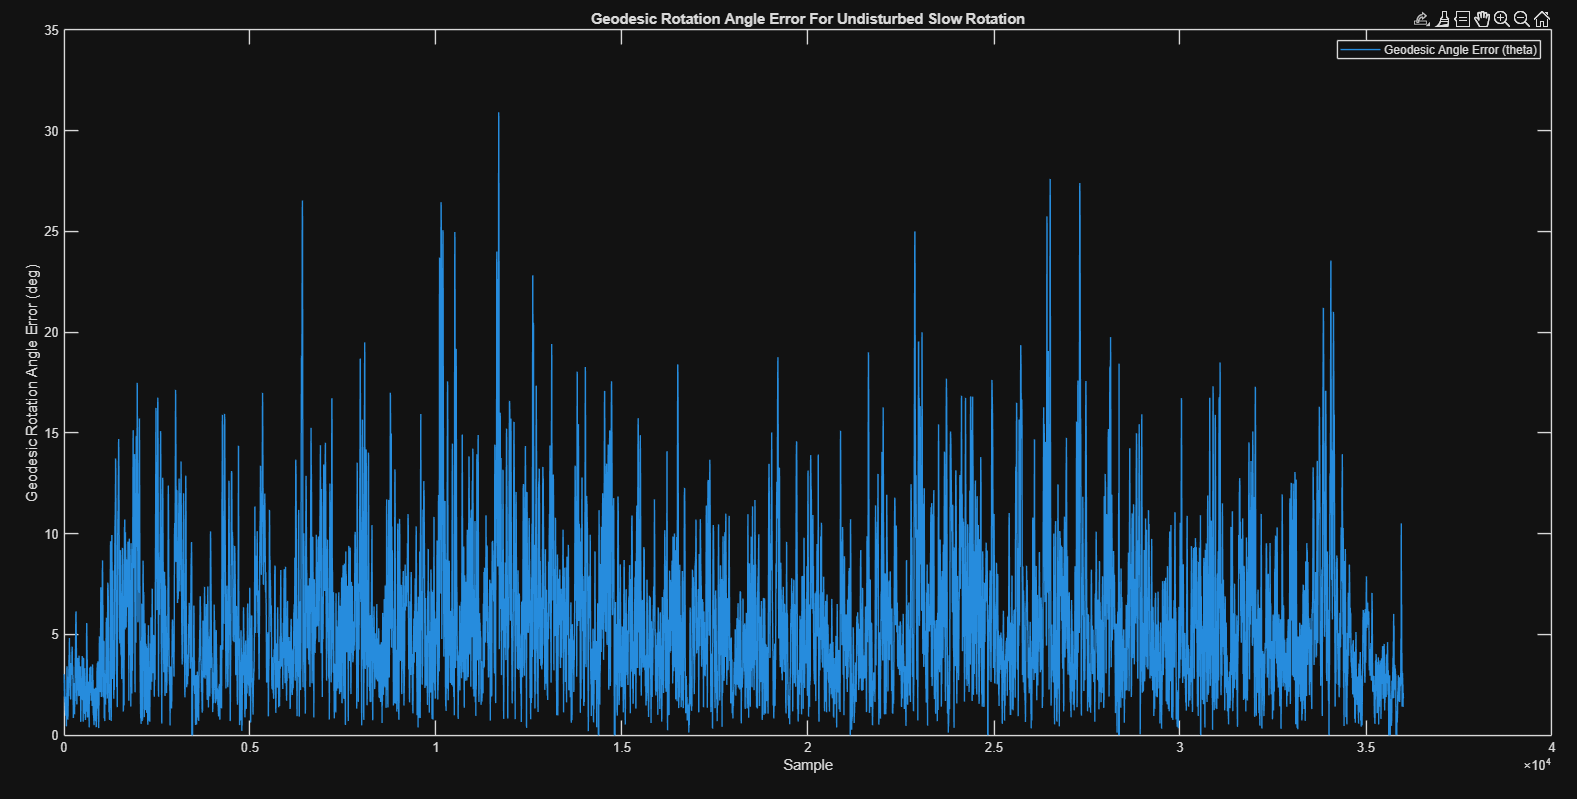
\includegraphics[width=15cm]{./figures/Data/geo1.png}
    \caption{Geodesic Angle Rotation Error for Undisturbed Slow Rotation}
    \label{fig:geo1}
\end{figure}

\begin{table}[!htbp]
\centering
\small
\begin{tabular}{p{3.0cm} p{3.0cm} p{3.0cm} p{3cm} p{3.0cm}}
\hline
\textbf{Mean ($\mu$)} & \textbf{Standard Deviation ($\sigma$)} & \textbf{Median}& \textbf{Minimum} & \textbf{Maximum} \\
\hline
$5.8150$
&
$3.7535$
&
$4.9821$
&
$0$
&
$30.9128$ \\
\hline
\end{tabular}
\caption{Summary of geodesic angle error $\theta$ for undisturbed slow rotation}
\label{tab:geo1}
\end{table}

\FloatBarrier

As we can see from the graph and table, the UKF performed reasonably well in determining the orientation
with a $\mu = 5.8150$, $\sigma = 3.7535$, and a $\text{median} = 4.9821$. This means that under undisturbed conditions of the
magnetometer and accelerometer, it is a viable choice to use a UKF to determine the orientation. 
Additionally, with a $\text{max} = 30.9128$, even though it is quite high under these close to
ideal conditions, the spikes were brief and the UKF was able to recover quite well to keep the mean low. 

The error is still not very close to 0, under these conditions. This can be due to multiple factors
including, gyroscopic drift caused by integration, the process and measurement noise not accurately 
modelling the sensors dynamics, and any misalignments in sensor axes. 


\subsubsection{Undisturbed Fast Rotation}

Undisturbed fast rotation refers to the test BROAD had done under an undisturbed magnetic field
and a fast rotation so there is high linear acceleration. Figure 4 and Table 3 shows a summary
of the geodesic angle error from the UKF.

\begin{figure}[H]
    \centering
    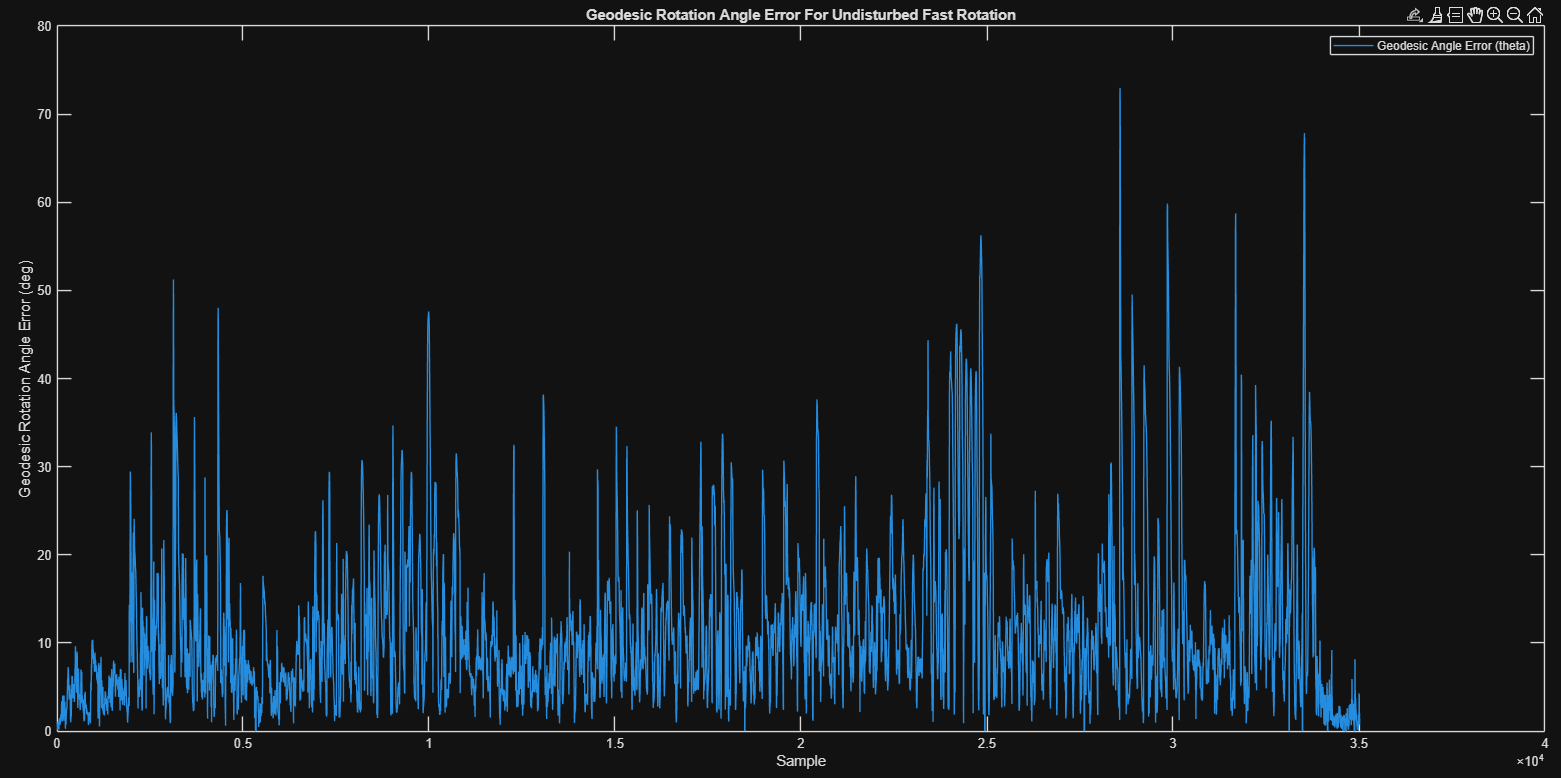
\includegraphics[width=15cm]{./figures/Data/geo2.png}
    \caption{Geodesic Angle Rotation Error for Undisturbed Fast Rotation}
    \label{fig:geo2}
\end{figure}

\begin{table}[!htbp]
\centering
\small
\begin{tabular}{p{3.0cm} p{3.0cm} p{3.0cm} p{3cm} p{3.0cm}}
\hline
\textbf{Mean ($\mu$)} & \textbf{Standard Deviation ($\sigma$)} & \textbf{Median}& \textbf{Minimum} & \textbf{Maximum} \\
\hline
$11.4535$
&
$9.0682$
&
$9.0273$
&
$0$
&
$72.9758$ \\
\hline
\end{tabular}
\caption{Summary of geodesic angle error $\theta$ for undisturbed fast rotation}
\label{tab:geo2}
\end{table}

\FloatBarrier

As we can see from the graph and table, the UKF performed okay in determining the orientation
with a $\mu = 11.4535$, $\sigma = 9.0682$, and a $\text{median} = 9.0273$. This means that under the
disturbed conditions of the accelerometer, the UKF is a reasonable choice, 
however, there is still a lot of room for improvement on the orientation estimation.  
Furthermore, with a $\text{max} = 72.9758$, this is very high and can lead to severe inaccuracies
if not addressed. Again, with the previous test, the UKF was able to recover relatively well but
this max would not be acceptable for an orientation of an object and can lead to severe consequences
if not addressed. 

\subsubsection{Disturbed Stationary Magnet}

Disturbed stationary magnet refers to the test BROAD had done under a disturbed magnetic field by
placing a stationary magnet next to the IMU, and medium-speed rotation so there is medium linear acceleration. 
Figure 5 and Table 4 shows a summary
of the geodesic angle error from the UKF.

\begin{figure}[H]
    \centering
    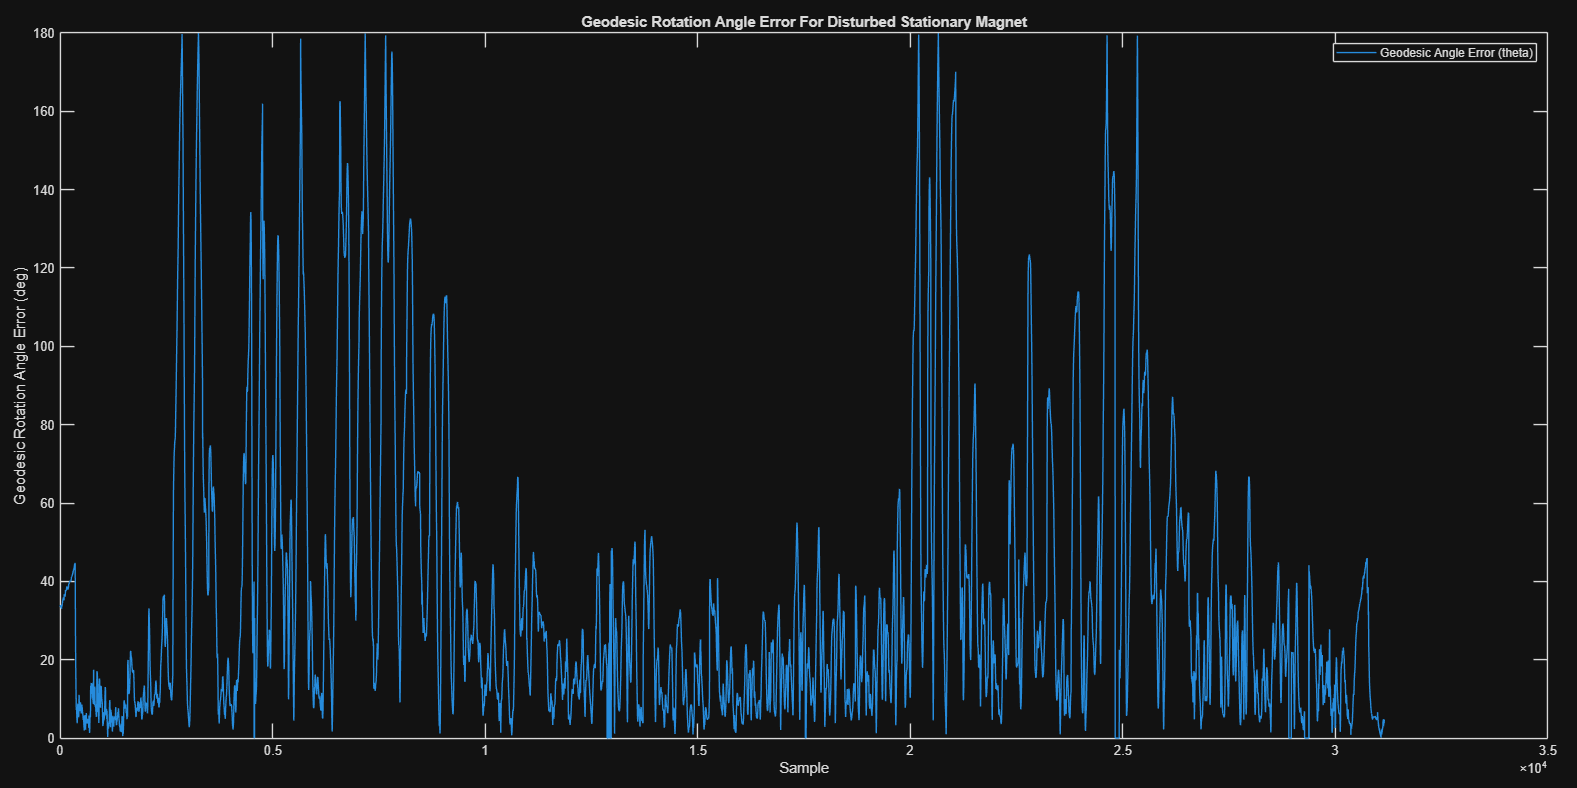
\includegraphics[width=15cm]{./figures/Data/geo3.png}
    \caption{Geodesic Angle Rotation Error for Disturbed Stationary Magnet}
    \label{fig:geo3}
\end{figure}

\begin{table}[!htbp]
\centering
\small
\begin{tabular}{p{3.0cm} p{3.0cm} p{3.0cm} p{3cm} p{3.0cm}}
\hline
\textbf{Mean ($\mu$)} & \textbf{Standard Deviation ($\sigma$)} & \textbf{Median}& \textbf{Minimum} & \textbf{Maximum} \\
\hline
$37.8035$
&
$38.8809$
&
$23.6325$
&
$0$
&
$179.9404$ \\
\hline
\end{tabular}
\caption{Summary of geodesic angle error $\theta$ for disturbed stationary magnet}
\label{tab:geo3}
\end{table}

\FloatBarrier

As we can see from the graph and table, the UKF performed terribly in determining the orientation
with a $\mu = 37.8035$, $\sigma = 38.8809$, and a $\text{median} = 23.6325$. This means that under
a magnetic disturbance, a UKF alone cannot be used for accurate orientation estimates even with
adaptive gating for the magnetometer. As the gating for the magnetometer would have likely 
downweighted the magnetic reference, the accumulation of errors through integration would have
also played a large role in the inaccuracy of the orientation.  

\newpage
\begin{figure}[H]
    \centering
    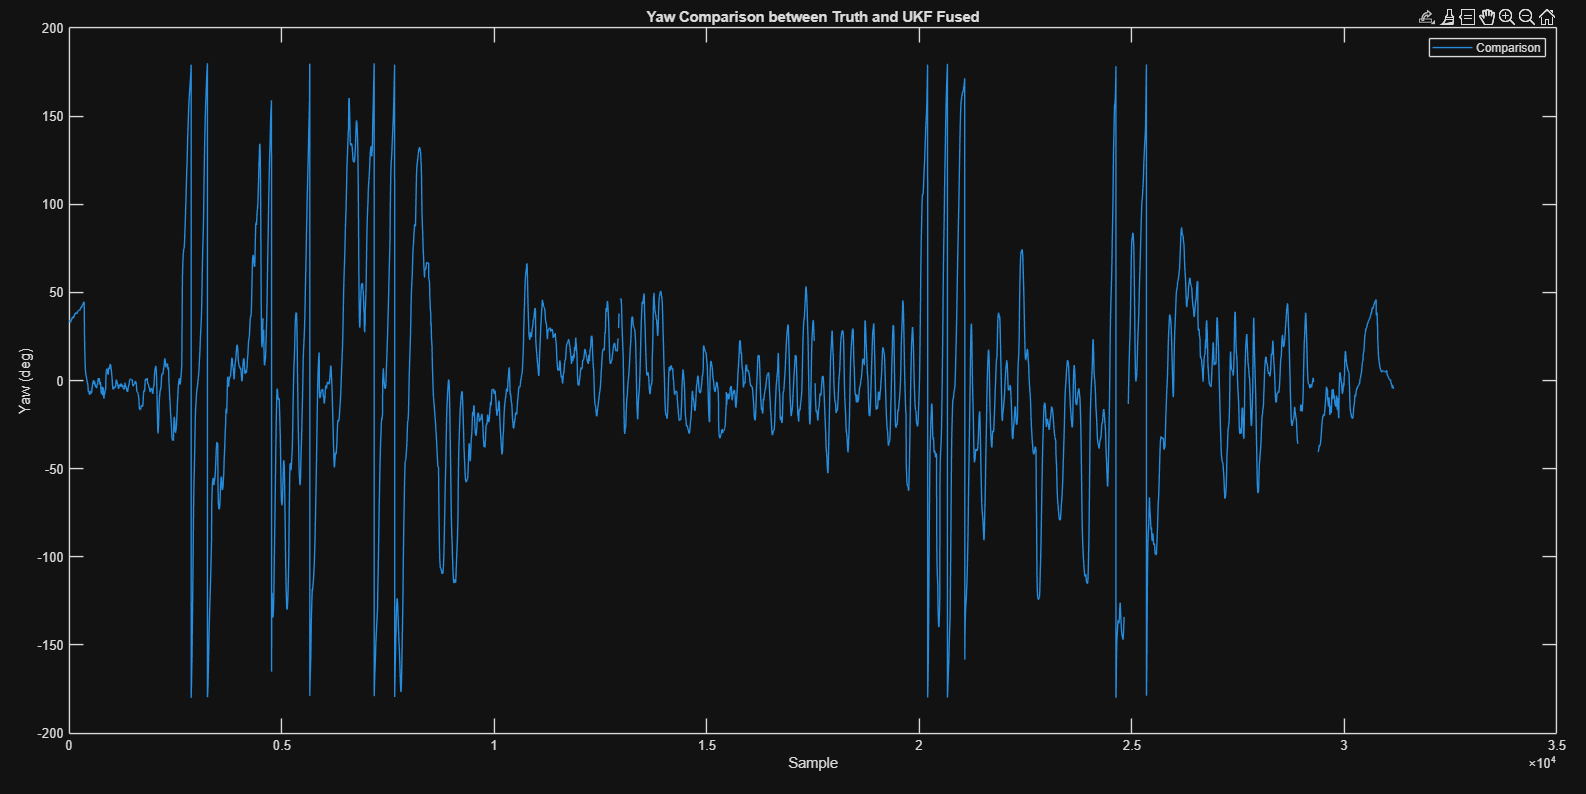
\includegraphics[width=15cm]{./figures/Data/yaw.png}
    \caption{Comparison of Yaw between Ground Truth and UKF fusion for Disturbed Stationary Magnet}
    \label{fig:yaw}
\end{figure}

This can be further shown by looking at the comparison of the yaw between ground truth and fusion.
Looking at Figure 6, we can see that the magnetic disturbance causes wide variations of the yaw
throughout the test. This further supports the conclusion that without addressing gyroscopic drift
through deep-learning, accurate orientation estimates from an IMU is unlikely.



